\documentclass[letter,11pt]{article}

\usepackage[spanish,es-nodecimaldot]{babel}
\usepackage[utf8]{inputenc}

\usepackage{lmodern}
\usepackage[T1]{fontenc}
\usepackage{textcomp}

\usepackage{framed}
\usepackage[svgnames]{xcolor}
\colorlet{shadecolor}{Gainsboro!50}

\usepackage[labelfont=bf]{caption}
\usepackage{graphicx}
\usepackage{pstricks}

\usepackage{anysize}
\marginsize{3cm}{2cm}{2cm}{3cm}

\usepackage{siunitx}
\usepackage{amsmath}
\usepackage{array}

\usepackage{fancyhdr}
\usepackage{lastpage}
\pagestyle{fancy}
\fancyhf{}
\fancyhead[LE,RO]{Laboratorio de Física Básica III}
\fancyfoot[CO,CE]{\thepage\ de \pageref{LastPage}}

\special{papersize=215.9mm,279.4mm}

\usepackage[
    pdfauthor={
        Bastos Lizondo Rosemary;
        Blanco Alconz John Brandon;
        Caballero Burgoa Carlos Eduardo;
        Villena Gutiérrez Ismael Cristian
    },%
    pdftitle={Laboratorio de Física Básica III},%
    pdfsubject={Campos magnéticos estacionarios},%
    colorlinks,%
    citecolor=black,%
    filecolor=black,%
    linkcolor=black,%
    urlcolor=black,
    breaklinks]{hyperref}
\usepackage{breakurl}

\newcommand{\blankpage}{
\newpage
\thispagestyle{empty}
\mbox{}
\newpage
}

\renewcommand{\arraystretch}{1.2}

\begin{document}

\begin{titlepage}
\begin{center}
{\Large UNIVERSIDAD MAYOR DE SAN SIMÓN}\\
\vspace*{0.15cm}
{\large FACULTAD DE CIENCIAS Y TECNOLOGÍA}\\
\vspace*{0.10cm}
DEPARTAMENTO DE FÍSICA\\
\vspace*{3.0cm}
{\Large \textbf{LABORATORIO DE FÍSICA BÁSICA III}}\\
\vspace*{0.3cm}
{\Large \textbf{INFORME No. 8}}\\
\vspace*{3.5cm}
{\Large \textbf{CAMPOS MAGNÉTICOS ESTACIONARIOS}}\\
\end{center}

\vspace*{5.8cm}
\leftskip=7.95cm
\noindent
\textbf{Integrantes:}\\
Bastos Lizondo Rosemary.\\
Blanco Alconz John Brandon.\\
Caballero Burgoa Carlos Eduardo.\\
Villena Gutiérrez Ismael Cristian.\\
\newline
\textbf{Docente:}\\
Ing. Flores Flores, Freddy.\\
\newline
\textbf{Grupo:} G3.\\
\textbf{Fecha de entrega:} 10 de Junio del 2021.\\

\end{titlepage}

\section{Evaluación previa}
\begin{enumerate}
\item \textbf{¿Cómo se producen campos magnéticos estacionarios?} \\
Los campos magnéticos estacionarios se generan mediante un imán o mediante
cargas que se mueven como un flujo constante.

\item \textbf{¿A partir de la ley de \emph{Ampère}, calcular el campo magnético
producido por un conductor rectilíneo infinito?} \\
La dirección del campo en un punto $P$, es perpendicular al plano determinado
por la corriente y el punto.

Se escoge como camino cerrado una circunferencia de radio $r$, centrada en la
corriente rectilínea y situada en un plano perpendicular a la misma.

El campo magnético $B$ es tangente a la circunferencia de radio $r$, paralelo al
vector $dl$.

El módulo del campo magnético $B$ tiene el mismo valor en todos los puntos de
dicha circunferencia.

La circulación (el primer miembro de la ley de \emph{Ampère}) vale:

\begin{equation*}
\oint \vec{B}\cdot\vec{dl}=\oint B\cdot dl cos (0) = B \oint dl = B\cdot2\pi\,R
\end{equation*}

La corriente rectilínea $i$ atraviesa la circunferencia de radio $r$.

Se despeja el módulo del campo magnético $B$.

\begin{equation*}
    B 2\pi R = \mu_0 i
\end{equation*}
\begin{equation*}
    B = \frac{\mu_0 i}{2\pi R}
\end{equation*}

\item \textbf{¿Cómo se puede generar un campo magnético uniforme?} \\
Se puede crear un campo magnético uniforme haciendo una bobina cilíndrica
relativamente larga. Una vez que la corriente fluye a través de la bobina,
existirá un campo magnético uniforme a lo largo del interior de la bobina. Esto
no es cierto en los extremos de la bobina.

Las bobinas de \emph{Helmholtz} pueden proporcionar un campo magnético
uniforme.

\item \textbf{¿Con qué instrumento se mide el campo magnético?} \\
Los medidores de campo magnético o gaussimetros son instrumentos para medir la
influencia magnética de las corrientes eléctricas y los campos magnéticos
producidos. Las unidades de medida utilizadas comúnmente para los medidores de
campo magnético son los tesla o los \emph{Gauss}.

\item \textbf{¿Qué es una bobina?} \\
Las bobinas son un elemento pasivo de dos terminales capaz de generar un flujo
magnético cuando se hace circular una corriente eléctrica.

Las bobinas están conformadas por un alambre o hilo de cobre esmaltado enrollado
en un núcleo, estos núcleos pueden tener diferente composición ya sea al aire o
en un material ferroso como por ejemplo acero magnético para intensificar su
capacidad de magnetismo.

\item \textbf{Calcular el campo magnético en la región central de una bobina.}
\\
Para calcular el campo magnético en la región central de una bobina se utiliza
la ecuación de \emph{Biot-Savart} la cual sirve para calcular el campo
magnético generado por cualquier elemento de corriente $d\vec{s}$.

Resultando ser:

\begin{equation*}
    \vec{B} = \frac{\mu_0 I r^2}{2 (r^2+d^2)^{3/2}} \hat{i}
\end{equation*}

Donde: \\
$\mu_0$, es la permeabilidad magnética del vacío. \\
$I$, es la corriente eléctrica circulante. \\
$r$, es el radio de la espira. \\
$d$, es la distancia desde el centro de la espira. \\

\item \textbf{¿Cómo se determina la polaridad del campo magnético producido por
una bobina?} \\
Cuando se conoce la dirección en que circula la corriente, la polaridad del
campo magnético se puede determinar mediante la regla de la mano izquierda para
bobinas. Si se toma la bobina con la mano izquierda y los dedos que la envuelven
señalan la dirección del flujo de corriente, el pulgar apunta hacia el polo
norte.
\end{enumerate}

\section{Objetivos}
\begin{itemize}
\item Determinar la relación funcional entre la magnitud de campo magnético $B$
y la distancia $r$ del centro de la espira sobre el eje del mismo.
\item Encontrar el valor de la permeabilidad magnética del vacío $\mu_0$
multiplicado por la corriente eléctrica $I$.
\end{itemize}

\section{Fundamento teórico}
El campo magnético $B$ es una campo vectorial, y a diferencia de las lineas de
campo eléctrico, las lineas de campo magnético son cerradas, y los vectores $B$
son tangentes a dichas lineas.

\begin{figure}[!h]
\centering
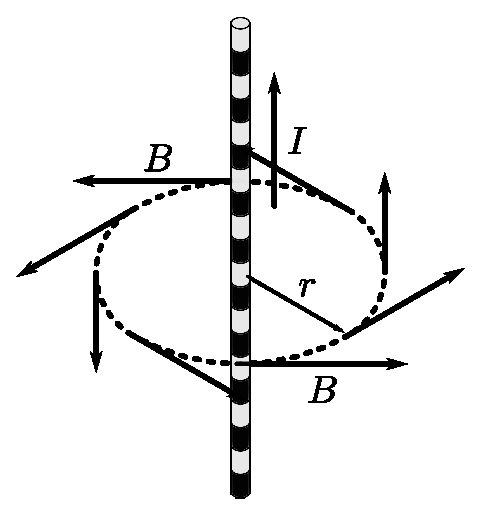
\includegraphics[scale=0.75]{resources/f1.eps}
\caption{Linea de campo magnético.}
\label{figura1}
\end{figure}

En la \textbf{Figura \ref{figura1}} se observa una linea de campo magnético
producida por un conductor rectilíneo infinito, por el cual circula una
corriente eléctrica constante $I$. La dirección del campo magnético está dada
por la regla de la mano derecha, y su valor puede ser calculado a partir de la
ley de \emph{Ampère}:

\begin{equation}
    \oint B \cdot dr = \mu_0\,I
\end{equation}

Donde: \\
$\mu_0 = \num{4\pi e-7} [N/A^2]$, es la permeabilidad magnética del vacío.

El módulo de un campo magnético estacionario a una distancia $r$ es:

\begin{equation}
    B = \frac{\mu_0 I}{2\pi r}
\end{equation}

\subsection{Campo magnético creado una espira circular}

\begin{figure}[!h]
\centering
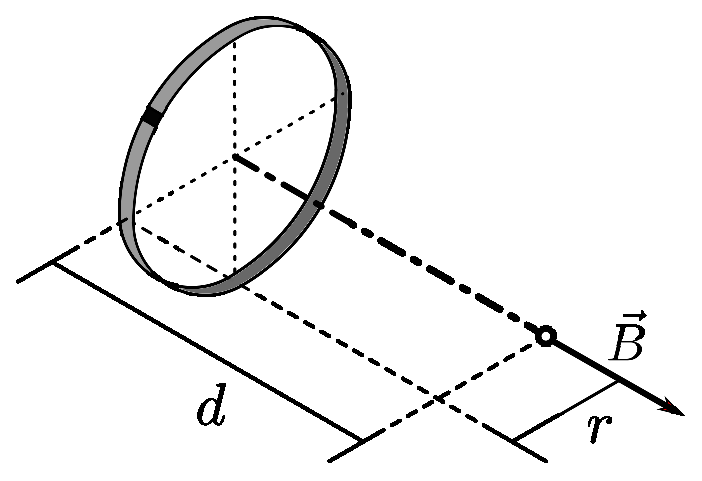
\includegraphics[scale=0.75]{resources/f2.eps}
\caption{Espira que genera un campo magnético.}
\label{figura2}
\end{figure}

Para el calculo del campo magnético de un alambre circular o espira como el
presentado en la \textbf{Figura \ref{figura2}}, se usa la ecuación de
\emph{Biot-Savart}:

\begin{equation*}
    \vec{B} = \frac{\mu_0 I}{4\pi} \int \frac{d\vec{s} \times \vec{r}}{r^2}
\end{equation*}

Cuyo resultado es:

\begin{equation}
    B = \frac{\mu_0 I r^2}{2 (r^2+d^2)^{3/2}}
\label{espira}
\end{equation}

Donde: \\
$\mu_0$, es la permeabilidad magnética del vacío. \\
$I$, es la corriente eléctrica circulante. \\
$r$, es el radio de la espira. \\
$d$, es la distancia desde el centro de la espira. \\

\section{Materiales}
\begin{itemize}
\item Simulador «PhET Interactive Simulations» Magnets and Electromagnets
(2.07.01).
\end{itemize}

\section{Procedimiento experimental}

A continuación se describe el procedimiento experimental que se llevará a cabo.

\begin{figure}[!h]
\centering
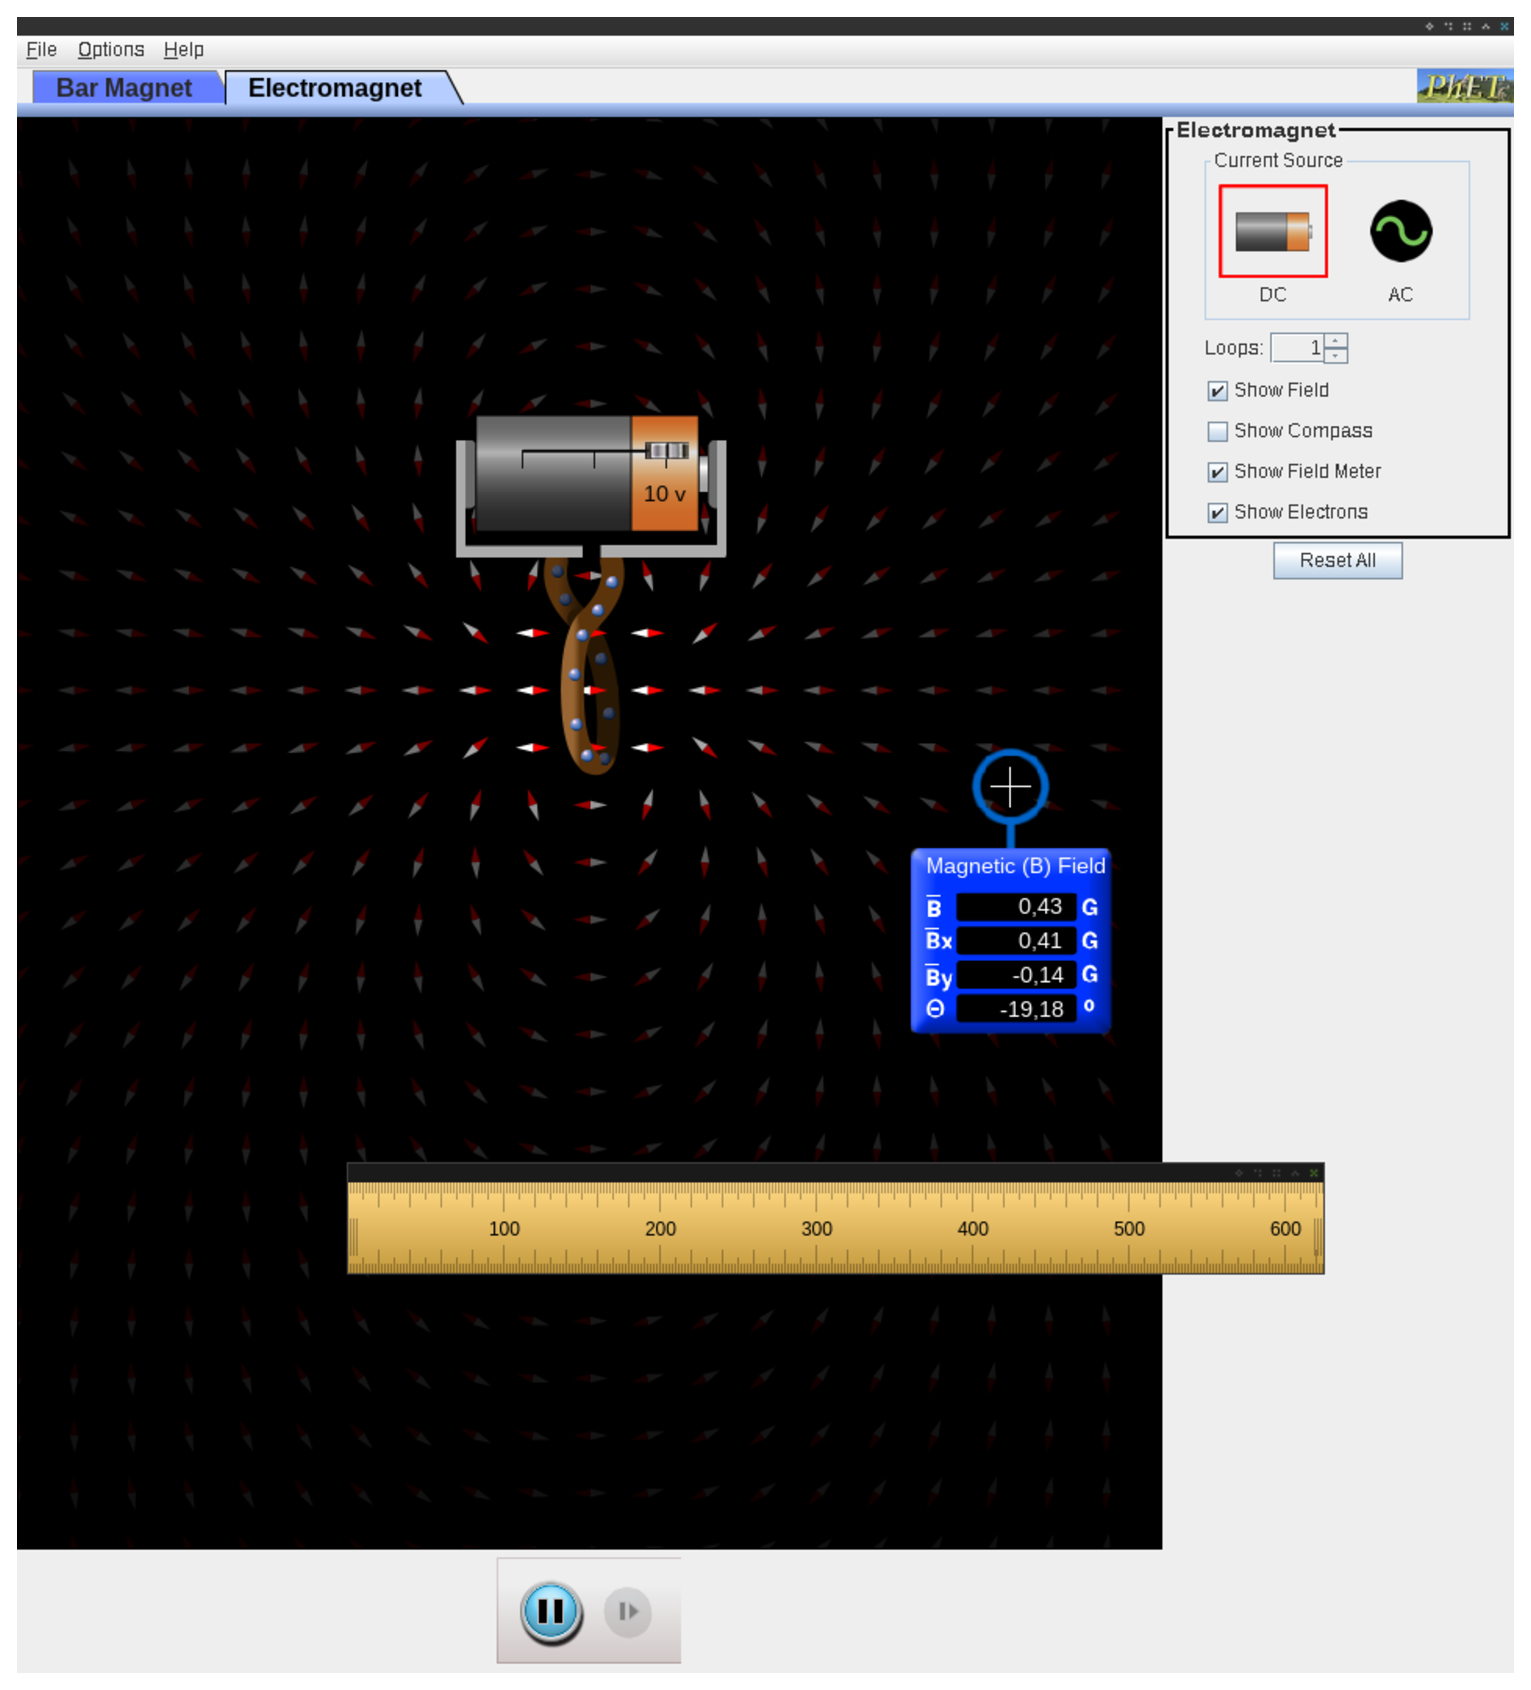
\includegraphics[scale=0.56]{resources/f3.eps}
\caption{Simulador de imanes y electroimanes.}
\label{figura3}
\end{figure}

\begin{enumerate}
\item Ir al simulador ubicado en la dirección web: (
\url{https://phet.colorado.edu/sims/cheerpj/faraday/latest/faraday.html?simulation=magnets-and-electromagnets}
), tal como se muestra en la \textbf{Figura \ref{figura3}}.
\item Establecer el valor de voltaje de la batería.
\item Con ayuda de una regla registrar el valor del campo magnético para
diferentes distancias sobre el eje central de la espira.
\item Registrar las mediciones tomadas, elaborar las gráficas e interpretar los
resultados.
\end{enumerate}

\section{Resultados}

Voltaje de la batería:

\begin{equation*}
    V = 10.0 [V]
\end{equation*}

Radio de la espira:

\begin{equation*}
    r = 19 [u]
\end{equation*}

En el \textbf{Cuadro \ref{cuadro1}} se presentan los valores del campo magnético
($B$) y las distancias ($d$).

\begin{table}[!h]
\begin{center}
\begin{tabular}{|c||>{\centering}m{1.2cm}<{\centering}
                   |>{\centering}m{1.2cm}<{\centering}|
                |c||>{\centering}m{1.2cm}<{\centering}
                   |>{\centering}m{1.2cm}<{\centering}|
                |c||>{\centering}m{1.2cm}<{\centering}
                   |>{\centering}m{1.2cm}<{\centering}
                   |>{\centering}m{1.2cm}<{\centering}
                   |>{\centering}m{1.2cm}<{\centering}|}
\hline
$i$ & $d_i [u]$ & $B_i [G]$ & 
$i$ & $d_i [u]$ & $B_i [G]$ &
$i$ & $d_i [u]$ & $B_i [G]$ \tabularnewline \hline \hline
 1 &  50 & 63.77 & 11 & 150 & 2.63 & 21 & 250 & 0.57 \tabularnewline \hline
 2 &  60 & 39.27 & 12 & 160 & 2.17 & 22 & 260 & 0.51 \tabularnewline \hline
 3 &  70 & 24.89 & 13 & 170 & 1.81 & 23 & 270 & 0.46 \tabularnewline \hline
 4 &  80 & 16.75 & 14 & 180 & 1.54 & 24 & 280 & 0.41 \tabularnewline \hline
 5 &  90 & 12.17 & 15 & 190 & 1.31 & 25 & 290 & 0.37 \tabularnewline \hline
 6 & 100 &  8.87 & 16 & 200 & 1.11 & 26 & 300 & 0.33 \tabularnewline \hline
 7 & 110 &  6.67 & 17 & 210 & 0.97 & 27 & 310 & 0.31 \tabularnewline \hline
 8 & 120 &  5.13 & 18 & 220 & 0.84 & 28 & 320 & 0.28 \tabularnewline \hline
 9 & 130 &  4.04 & 19 & 230 & 0.74 & 29 & 330 & 0.25 \tabularnewline \hline
10 & 140 &  3.23 & 20 & 240 & 0.65 &    &     &      \tabularnewline \hline
\end{tabular}
\caption{Mediciones de campo magnético y distancia del centro de la espira.}
\label{cuadro1}
\end{center}
\end{table}

\begin{figure}[!h]
\centering
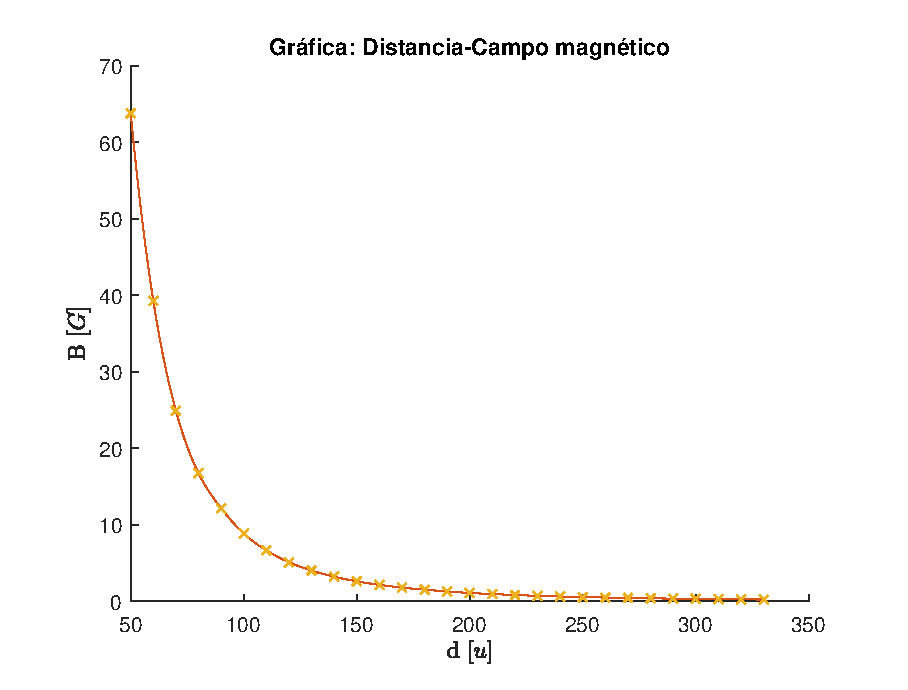
\includegraphics[scale=1.00]{resources/m1.1.eps}
\caption{Campo magnético en función de la distancia sobre el eje.}
\label{figura4}
\end{figure}

A partir de los datos del \textbf{Cuadro \ref{cuadro1}}, se obtiene la gráfica
presentada en la \textbf{Figura \ref{figura4}}.

Por la forma de la \textbf{Figura \ref{figura4}} y considerando la
\textbf{Ecuación \ref{espira}}:

\begin{equation*}
    B(d) = a d^b
\end{equation*}

Aplicando logaritmos a ambos lados de la ecuación obtenemos:

\begin{equation*}
    \log B = \log a + b \log d
\end{equation*}

Haciendo los siguientes cambios de variables:

\begin{equation*}
    B' = \log B
\end{equation*}
\begin{equation*}
    A = \log a
\end{equation*}
\begin{equation*}
    B = b
\end{equation*}
\begin{equation*}
    d' = \log (r^2+d^2)
\end{equation*}

Se obtiene:

\begin{equation*}
    B' = A + B d'
\end{equation*}

En el \textbf{Cuadro \ref{cuadro2}} pueden apreciarse los valores de la función
aplicando los cambios de variable respectivos, tales datos generan la gráfica
presentada en la \textbf{Figura \ref{figura5}}.

\begin{table}[!h]
\begin{center}
\begin{tabular}{|c||>{\centering}m{1.35cm}<{\centering}
                   |>{\centering}m{1.35cm}<{\centering}|
                |c||>{\centering}m{1.35cm}<{\centering}
                   |>{\centering}m{1.35cm}<{\centering}|
                |c||>{\centering}m{1.35cm}<{\centering}
                   |>{\centering}m{1.35cm}<{\centering}
                   |>{\centering}m{1.35cm}<{\centering}
                   |>{\centering}m{1.35cm}<{\centering}|}
\hline
$i$ & $d'_i$ & $B'_i$ & 
$i$ & $d'_i$ & $B'_i$ &
$i$ & $d'_i$ & $B'_i$ \tabularnewline \hline \hline
 1 & 7.9589 & 4.1553 & 11 & 10.0372 &  0.9670 & 21 & 11.0487 & -0.5621 \tabularnewline \hline
 2 & 8.2843 & 3.6705 & 12 & 10.1644 &  0.7747 & 22 & 11.1267 & -0.6733 \tabularnewline \hline
 3 & 8.5681 & 3.2145 & 13 & 10.2840 &  0.5933 & 23 & 11.2018 & -0.7765 \tabularnewline \hline
 4 & 8.8189 & 2.8184 & 14 & 10.3970 &  0.4318 & 24 & 11.2742 & -0.8916 \tabularnewline \hline
 5 & 9.0432 & 2.4990 & 15 & 10.5040 &  0.2700 & 25 & 11.3440 & -0.9943 \tabularnewline \hline
 6 & 9.2458 & 2.1827 & 16 & 10.6056 &  0.1044 & 26 & 11.4116 & -1.1087 \tabularnewline \hline
 7 & 9.4304 & 1.8976 & 17 & 10.7024 & -0.0305 & 27 & 11.4769 & -1.1712 \tabularnewline \hline
 8 & 9.5997 & 1.6351 & 18 & 10.7947 & -0.1744 & 28 & 11.5402 & -1.2730 \tabularnewline \hline
 9 & 9.7562 & 1.3962 & 19 & 10.8830 & -0.3011 & 29 & 11.6015 & -1.3863 \tabularnewline \hline
10 & 9.9015 & 1.1725 & 20 & 10.9675 & -0.4308 &    &         &         \tabularnewline \hline
\end{tabular}
\caption{Valores después del cambio de variable.}
\label{cuadro2}
\end{center}
\end{table}

\begin{figure}[!h]
\centering
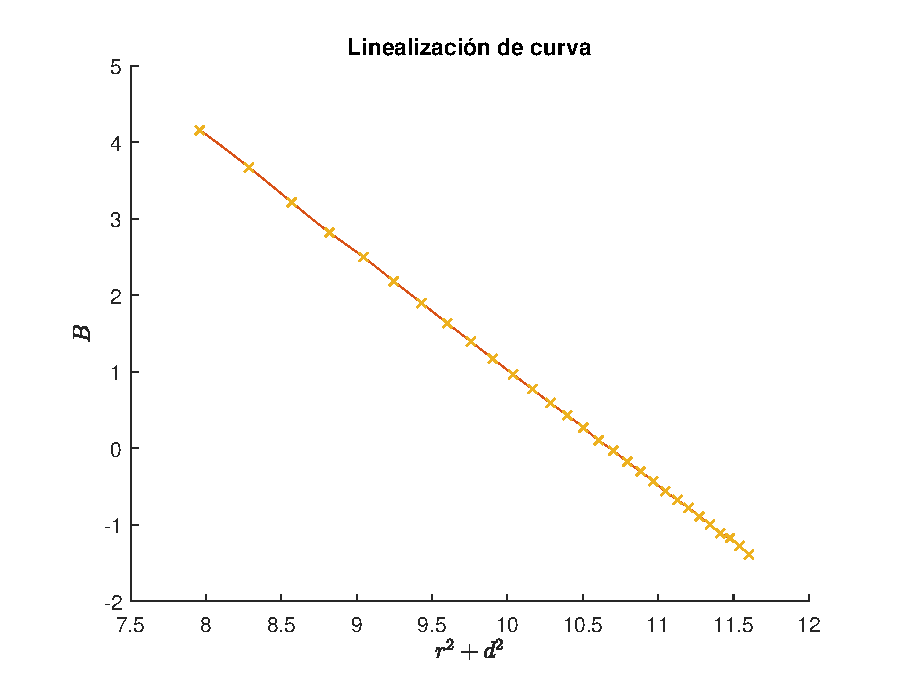
\includegraphics[scale=1.00]{resources/m1.2.eps}
\caption{Gráfica de la función linealizada.}
\label{figura5}
\end{figure}

Se calcularon los parámetros de la recta por el método de los mínimos cuadrados,
con la ayuda de los datos presentados en el \textbf{Cuadro \ref{cuadro3}}.

\begin{table}[!h]
\begin{center}
\begin{tabular}{|c||>{\centering}m{1.6cm}<{\centering}
                   |>{\centering}m{1.6cm}<{\centering}
                   |>{\centering}m{1.6cm}<{\centering}|
                   |>{\centering}m{1.8cm}<{\centering}
                   |>{\centering}m{1.8cm}<{\centering}
                   |>{\centering}m{1.8cm}<{\centering}|}
\hline
$i$ & $d'_i B'_i$ & $d'^2_i$ & $B'^2_i$ & $Y$ & $d_i$ & $d^2_i (\num{e-5})$
    \tabularnewline \hline \hline
 1 &  63.3445 & 17.2664 &  33.0716 &  4.1355 &  0.0198 & 0.0004 \tabularnewline \hline
 2 &  68.6288 & 13.4723 &  30.4070 &  3.6418 &  0.0286 & 0.0008 \tabularnewline \hline
 3 &  73.4119 & 10.3328 &  27.5418 &  3.2111 &  0.0033 & 0.0000 \tabularnewline \hline
 4 &  77.7735 &  7.9434 &  24.8552 &  2.8305 & -0.0121 & 0.0001 \tabularnewline \hline
 5 &  81.7799 &  6.2449 &  22.5988 &  2.4901 &  0.0089 & 0.0001 \tabularnewline \hline
 6 &  85.4849 &  4.7641 &  20.1806 &  2.1827 &  0.0000 & 0.0000 \tabularnewline \hline
 7 &  88.9317 &  3.6010 &  17.8952 &  1.9026 & -0.0050 & 0.0000 \tabularnewline \hline
 8 &  92.1551 &  2.6736 &  15.6966 &  1.6456 & -0.0105 & 0.0001 \tabularnewline \hline
 9 &  95.1835 &  1.9495 &  13.6220 &  1.4081 & -0.0119 & 0.0001 \tabularnewline \hline
10 &  98.0404 &  1.3747 &  11.6094 &  1.1876 & -0.0151 & 0.0002 \tabularnewline \hline
11 & 100.7451 &  0.9351 &   9.7058 &  0.9817 & -0.0148 & 0.0002 \tabularnewline \hline
12 & 103.3140 &  0.6002 &   7.8746 &  0.7888 & -0.0140 & 0.0002 \tabularnewline \hline
13 & 105.7609 &  0.3520 &   6.1018 &  0.6072 & -0.0139 & 0.0002 \tabularnewline \hline
14 & 108.0975 &  0.1864 &   4.4892 &  0.4357 & -0.0040 & 0.0000 \tabularnewline \hline
15 & 110.3340 &  0.0729 &   2.8364 &  0.2734 & -0.0033 & 0.0000 \tabularnewline \hline
16 & 112.4792 &  0.0109 &   1.1068 &  0.1192 & -0.0148 & 0.0002 \tabularnewline \hline
17 & 114.5407 &  0.0009 &  -0.3260 & -0.0277 & -0.0028 & 0.0000 \tabularnewline \hline
18 & 116.5252 &  0.0304 &  -1.8821 & -0.1678 & -0.0066 & 0.0000 \tabularnewline \hline
19 & 118.4388 &  0.0907 &  -3.2769 & -0.3017 &  0.0006 & 0.0000 \tabularnewline \hline
20 & 120.2866 &  0.1856 &  -4.7246 & -0.4300 & -0.0007 & 0.0000 \tabularnewline \hline
21 & 122.0734 &  0.3160 &  -6.2107 & -0.5532 & -0.0089 & 0.0001 \tabularnewline \hline
22 & 123.8032 &  0.4534 &  -7.4921 & -0.6716 & -0.0018 & 0.0000 \tabularnewline \hline
23 & 125.4800 &  0.6030 &  -8.6985 & -0.7855 &  0.0090 & 0.0001 \tabularnewline \hline
24 & 127.1070 &  0.7949 & -10.0520 & -0.8954 &  0.0038 & 0.0000 \tabularnewline \hline
25 & 128.6874 &  0.9885 & -11.2788 & -1.0014 &  0.0072 & 0.0001 \tabularnewline \hline
26 & 130.2239 &  1.2291 & -12.6516 & -1.1039 & -0.0048 & 0.0000 \tabularnewline \hline
27 & 131.7191 &  1.3717 & -13.4415 & -1.2030 &  0.0318 & 0.0010 \tabularnewline \hline
28 & 133.1753 &  1.6204 & -14.6902 & -1.2990 &  0.0260 & 0.0007 \tabularnewline \hline
29 & 134.5947 &  1.9218 & -16.0831 & -1.3921 &  0.0058 & 0.0000 \tabularnewline \hline
\end{tabular}
\caption{Valores para el método de mínimos cuadrados.}
\label{cuadro3}
\end{center}                                                   
\end{table}

\begin{equation*}
    n = 29
\end{equation*}
\begin{equation*}
    \sum d'_i = 297.9722
\end{equation*}
\begin{equation*}
    \sum B'_i = 18.0093
\end{equation*}
\begin{equation*}
    \sum d'^2_i = \num{3.0921e3}
\end{equation*}
\begin{equation*}
    \sum B'^2_i = 81.3865
\end{equation*}
\begin{equation*}
    \sum d'_i B'_i = 138.7846
\end{equation*}
\begin{equation*}
    \Delta_1 = n \sum d'^2_i - \left( \sum d'_i \right)^2 = 884.0252
\end{equation*}
\begin{equation*}
    \Delta_2 = n \sum B'^2_i - \left( \sum B'_i \right)^2 = \num{2.0359e3}
\end{equation*}
\begin{equation*}
    A = \frac{\sum B'_i \sum d'^2_i - \sum d'_i B'_i \sum d'_i}{\Delta_1} = 16.2132
\end{equation*}
\begin{equation*}
    B = \frac{n \sum d'_i B'_i - \sum d'_i \sum B'_i}{\Delta_1} = -1.5175
\end{equation*}
\begin{equation*}
    \sum d'^2 = 0.0048
\end{equation*}
\begin{equation*}
    \sigma^2 = \frac{\sum d'^2_i}{n-2} = \num{1.7902e-4}
\end{equation*}
\begin{equation*}
    \sigma_A = \sqrt{\frac{\sigma^2 \sum d'^2_i}{\Delta_1}} = 0.0250
\end{equation*}
\begin{equation*}
    \sigma_B = \sqrt{\frac{\sigma^2 n}{\Delta_1}} = 0.0024
\end{equation*}

\begin{equation*}
    A = (16.21 \pm 0.02 )[u]; 0.15 \%
\end{equation*}
\begin{equation*}
    B = (-1.517 \pm 0.002)[u]; 0.16 \%
\end{equation*}

Siendo el coeficiente de correlación:

\begin{equation*}
    r = \frac{n \sum d'_i B'_i - (\sum d'_i)(\sum B'_i)}{\sqrt{\Delta_1 \Delta_2}} = -1.0000
\end{equation*}

A partir de los parámetros de recta $A$ y $B$, calculamos los parámetros $a$ y
$b$ de la curva original y sus errores por el método de propagación de errores:

\begin{equation*}
    a = e^A = e^{16.21} =  \num{1.0997e7}
\end{equation*}
\begin{equation*}
    b = B = -1.5
\end{equation*}
\begin{equation*}
    e_a = e^A e_A = e^{(16.21)} 0.0250 = \num{2.7519e5}
\end{equation*}
\begin{equation*}
    e_b = e_B = 0.0024
\end{equation*}

Obteniendo finalmente los valores de la curva:

\begin{equation*}
    a = (\num{1.0997e7} \pm \num{2.7519e5})[\text{Wb}-u]; 2.50\%
\end{equation*}
\begin{equation*}
    b = (-1.517 \pm 0.002)[u]; 0.16\%
\end{equation*}

Por tanto, se comprueba la relación entre el campo magnético y la distancia en
una espira descrito por la \textbf{Ecuación \ref{espira}}.

\begin{center}
\begin{tabular}{|>{\centering}m{9.2cm}<{\centering}|}
\hline
\textbf{Resultado} 
\tabularnewline \hline
\\
\Large{$B(d) \propto \dfrac{1}{(r^2+d^2)^{3/2}} $} \tabularnewline
\\
\hline
\end{tabular}
\end{center}

Se determinará el valor de $\mu_0 I$, a partir de la
\textbf{Ecuación \ref{espira}}:

\begin{equation*}
    a = \frac{\mu_0 I r^2}{2}
\end{equation*}
\begin{equation*}
    \mu_0 I = \frac{2a}{r^2} = \num{6.0927e4} [Wb/u]
\end{equation*}

La derivada parcial es:

\begin{equation*}
    \frac{\partial (\mu_0 I)}{\partial a} = \frac{2}{r^2}
\end{equation*}

Siendo el error de la medición:

\begin{equation*}
    e_{\mu_0 I} = \Biggr| \frac{2}{r^2}\,e_a \Biggr| = \num{1.5246e3}
\end{equation*}

Por tanto el valor de $\mu_0 I$ es:

\begin{center}
\begin{tabular}{|>{\centering}m{12.0cm}<{\centering}|}
\hline
\textbf{Resultado}
\tabularnewline \hline
\\
    $\mu_0 I = (60927 \pm 1525)[\text{Wb}/u]; 2.50\%$ \tabularnewline
\\
\hline
\end{tabular}
\end{center}

Lamentablemente el simulador carece de los datos suficientes para el calculo de
la corriente circulante, dato con el cual se podría calcular el valor de
$\mu_0$.

\end{document}

